\section{Systemtechnik}

\subsection{Modellbildung}
\begin{tcolorbox}
\boxtitle{Hinweise zum Aufstellen der Differentialgleichung (DGL)}
\begin{enumerate}
  \item \textbf{Bestimmung} der Ein- und Ausgangsgrößen.
  \item \textbf{Suche} nach dem beschreibenden physikalischen Gleichgewicht (Kräfte-, Momenten-, Knoten-, Maschenbilanz).
  \item In der Endgleichung dürfen nur Konstanten sowie die Ein- und Ausgangsgrößen in beliebiger Zeitableitung vorkommen.
  \item Alle Zwischenvariablen müssen durch physikalische Gesetze eliminiert werden.
\end{enumerate}
\end{tcolorbox}

\subsection{Signalflussplan / Blockschaltbild}
\begin{tcolorbox}
\boxtitle{Erzeugung des Signalflussplans aus der DGL}
\begin{enumerate}
  \item Für technische Realisierbarkeit gilt: $m \le n$ (Zählergrad $\le$ Nennergrad).
  \item DGL nach der höchsten Ableitung der Ausgangsgröße auflösen.
  \item Die höchste Ableitung der Ausgangsgröße wird auf den Eingang einer Kette von $n$ Integratoren ($1/s$) geführt.
\end{enumerate}
\end{tcolorbox}

\begin{center}
  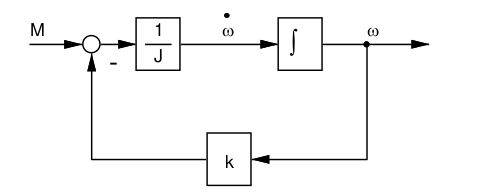
\includegraphics[width=0.95\columnwidth]{images/sfp_dgl_masse_feder.png}
\end{center}

\begin{tcolorbox}
\boxtitle{Signalflussplan eines Systems $n$-ter Ordnung mit DGL:}
\[
a_n x_a^{(n)} + \dots + a_1 \dot{x}_a + a_0 x_a = b_m x_e^{(m)} + \dots + b_1 \dot{x}_e + b_0 x_e
\]
\begin{center}
  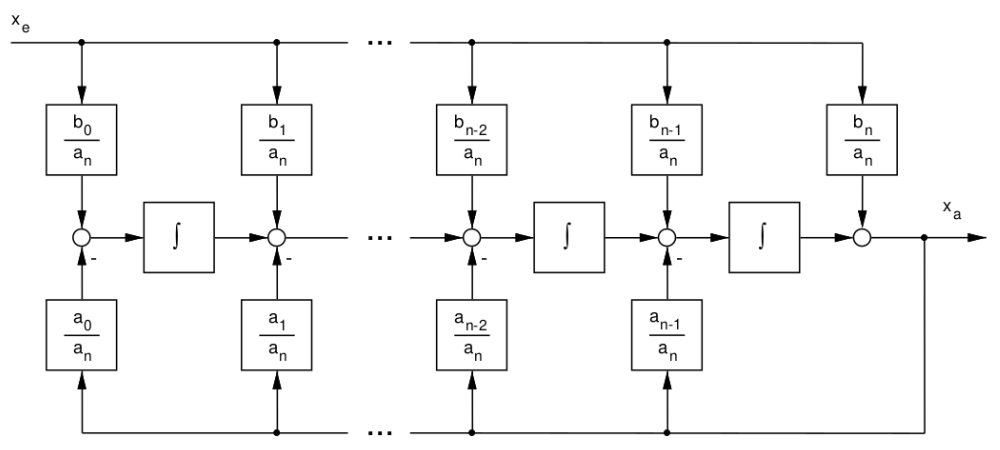
\includegraphics[width=\columnwidth]{images/sfp_dgl_ordnung.png}
\end{center}
Falls $m < n$, sind alle höheren Koeffizienten $b_\mu = 0$ zu setzen.
\end{tcolorbox}

\subsection{Übertragungsfunktion $F(s)$}
\begin{tcolorbox}
Definition bei verschwindenden Anfangsbedingungen:
\[
F(s) = \frac{\mathcal{L}\{x_a(t)\}}{\mathcal{L}\{x_e(t)\}} = \frac{X_a(s)}{X_e(s)}
\]
\end{tcolorbox}

\subsubsection{$F(s)$ aus der DGL}
\begin{tcolorbox}
\[
F(s) = \frac{b_m s^m + b_{m-1} s^{m-1} + \dots + b_1 s + b_0}{a_n s^n + a_{n-1} s^{n-1} + \dots + a_1 s + a_0}
\]
\end{tcolorbox}

\subsubsection{$F(s)$ in Pol- und Nullstellenform}
\begin{tcolorbox}
\[
F(s) = Q \cdot \frac{\prod_{\mu=1}^m (s - s_{N\mu})}{\prod_{\nu=1}^n (s - s_{P\nu})} \quad \text{mit } Q = \frac{b_m}{a_n}
\]
\textbf{Eigenschaften von Polen ($s_{P\nu}$):}
\begin{itemize}
  \item Pole in der rechten $s$-Halbebene ($\text{Re}\{s_P\} > 0$) führen zu einem \textbf{instabilen} System. Sie können \textbf{nicht} durch Nullstellen kompensiert werden!
  \item Pole bewirken verzögerndes Verhalten. Je weiter links sie in der komplexen Ebene liegen, desto schneller klingt der Einschwingvorgang ab.
  \item Liegen Pole deutlich weiter links als dominante Pole, können sie meist ohne großen Fehler vernachlässigt werden.
\end{itemize}
\textbf{Eigenschaften von Nullstellen ($s_{N\mu}$):}
\begin{itemize}
  \item Nullstellen bewirken differenzierendes Verhalten (Vorhalt, Phasendrehung nach oben, Beschleunigung des Systems).
  \item Nullstellen weit links in der $s$-Ebene haben geringen Einfluss.
\end{itemize}
\end{tcolorbox}

\subsection{Signalflussplan-Algebra}

\begin{tcolorbox}
\boxtitle{Kettenstruktur (Reihenschaltung)}
\begin{center}
  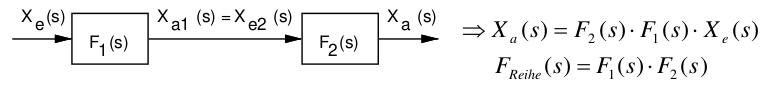
\includegraphics[width=0.9\columnwidth]{images/sfp_reihe.png}
\end{center}
\[
X_a(s) = F_2(s) \cdot F_1(s) \cdot X_e(s) \implies F_{\text{Reihe}}(s) = F_1(s) \cdot F_2(s)
\]
\end{tcolorbox}

\begin{tcolorbox}
\boxtitle{Parallelstruktur (Parallelschaltung)}
\begin{center}
  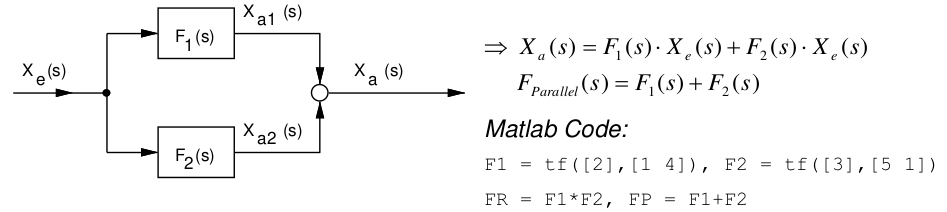
\includegraphics[width=0.9\columnwidth]{images/sfp_parallel.png}
\end{center}
\[
F_{\text{Parallel}}(s) = F_1(s) + F_2(s)
\]
\end{tcolorbox}

\begin{tcolorbox}
\boxtitle{Kreisstruktur (Rückkopplung)}
\begin{center}
  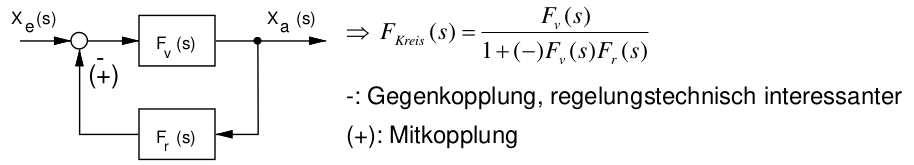
\includegraphics[width=0.75\columnwidth]{images/sfp_kreis.png}
\end{center}
\[
F_{\text{Kreis}}(s) = \frac{F_v(s)}{1 + F_v(s) \cdot F_r(s)} \quad \text{bei Gegenkopplung (-)}
\]
(Bei Mitkopplung (+) steht im Nenner $1 - F_v(s) F_r(s)$).
\end{tcolorbox}

\begin{tcolorbox}
\boxtitle{Verschieben einer Additionsstelle}
\begin{center}
  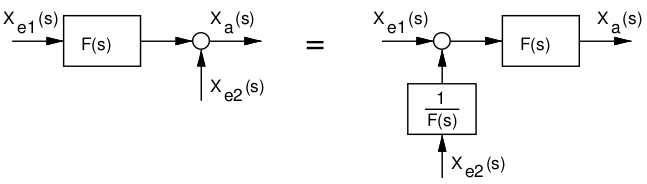
\includegraphics[width=\columnwidth]{images/sfp_addition_verschieben.png}
\end{center}
\end{tcolorbox}

\begin{tcolorbox}
\boxtitle{Verschieben einer Verzweigung}
\begin{center}
  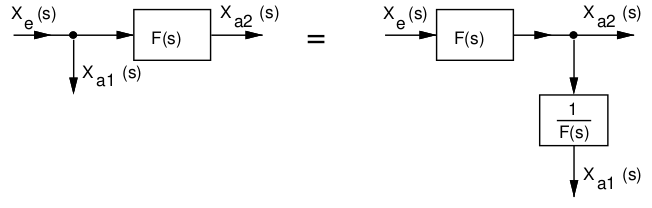
\includegraphics[width=\columnwidth]{images/sfp_verzweigung_verschieben.png}
\end{center}
\end{tcolorbox}

\subsection{Standard-Übertragungsglieder}
\begin{tcolorbox}
\small
\begin{tabularx}{\columnwidth}{l X X}
\toprule
\textbf{Typ} & \textbf{Übertragungsfunktion $F(s)$} & \textbf{Sprungantwort $h(t)$} \\
\midrule
\textbf{P} & $K_P$ & $K_P \cdot \sigma(t)$ \\[2pt]
\textbf{I} & $\frac{K_I}{s} = \frac{1}{T_I s}$ & $K_I \cdot t = \frac{t}{T_I}$ \\[2pt]
\textbf{D} & $K_D \cdot s = T_D s$ & $K_D \cdot \delta(t)$ \\[2pt]
\textbf{PT}$_1$ & $\frac{K}{1 + T s}$ & $K (1 - e^{-t/T})$ \\[2pt]
\textbf{PT}$_2$ & $\frac{K}{1 + \frac{2D}{\omega_0} s + \frac{s^2}{\omega_0^2}}$ & $K \left[1 - \frac{e^{-D\omega_0 t}}{\sqrt{1-D^2}} \sin(\omega_d t + \varphi)\right]$ \\[2pt]
\textbf{IT}$_1$ & $\frac{K_I}{s (1 + T s)}$ & $K_I [t - T(1 - e^{-t/T})]$ \\[2pt]
\textbf{DT}$_1$ & $\frac{K_D s}{1 + T s}$ & $\frac{K_D}{T} e^{-t/T}$ \\[2pt]
\textbf{T}$_t$ & $e^{-s T_t}$ & $\sigma(t - T_t)$ \\
\bottomrule
\end{tabularx}
\end{tcolorbox}
